\section*{Question 6}
\subsection*{(g)}
\graphicspath{{q6_expectation_maximization_python/}}
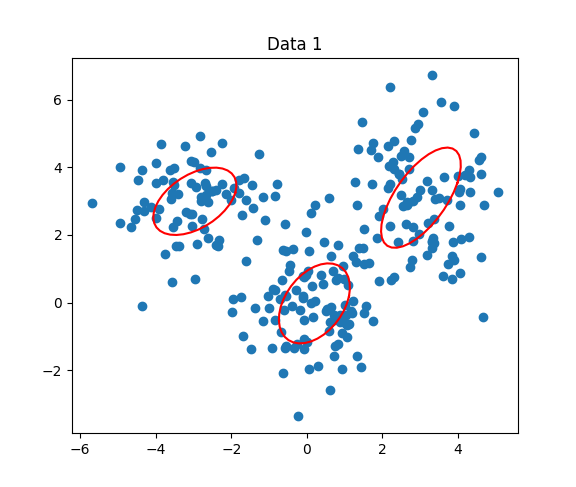
\includegraphics[width=0.5\textwidth]{Figure_1.png}
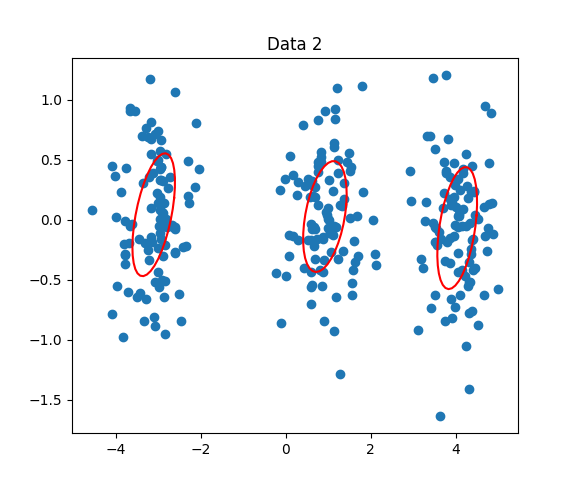
\includegraphics[width=0.5\textwidth]{Figure_2.png}
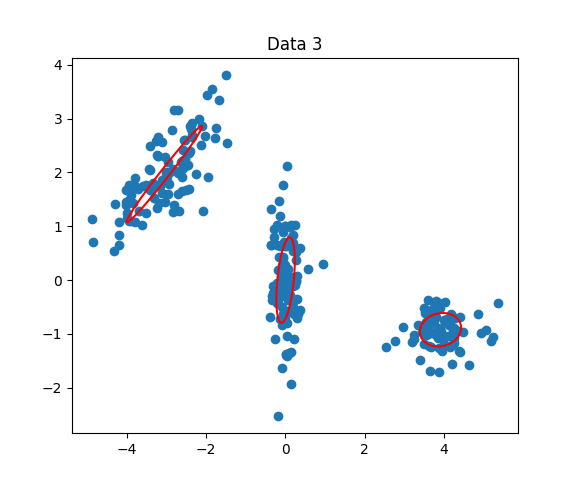
\includegraphics[width=0.5\textwidth]{Figure_3.png}
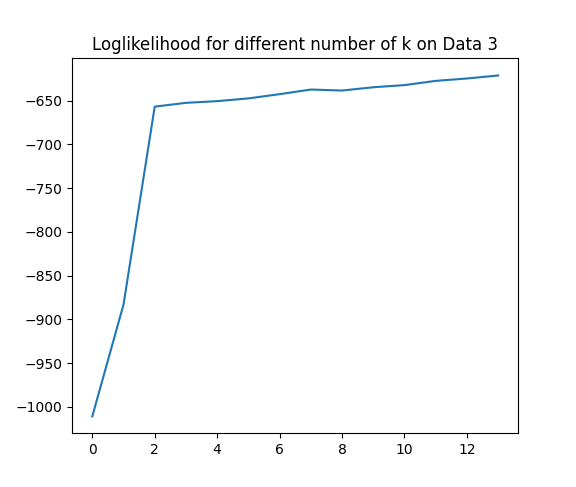
\includegraphics[width=0.5\textwidth]{Figure_4.png}

We can see, that in all three data sets there are 3 clusters (more so in data2 and data3 than in data1). Therefore, $K=3$ clusters is a very suitable number of clusters for this application.

$K=2$ yields very under fitting cluster parameters, even for data1. For $K>3$ we get clusters that are "overlapping" each other, so we see overfitting.


\subsection*{(h)}
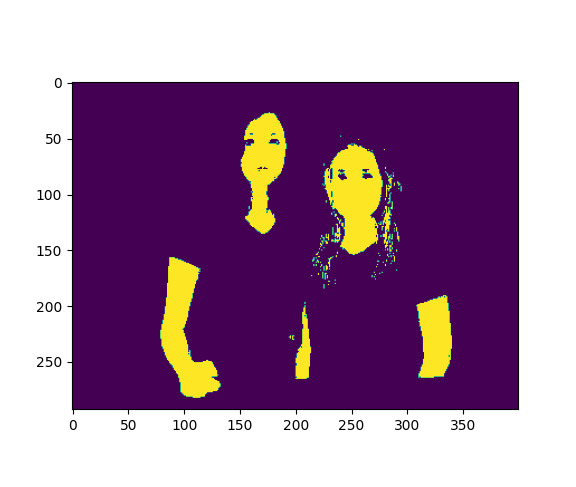
\includegraphics[width=0.5\textwidth]{Figure_5.png}

Increasing $K$ here improves accuracy on the training data set, thus reducing generalization. For $K=9$, a model is produced that separates the colors in the test image better than the default of $K=3$. Increasing $K$ further might lead to poor accuracy on other test data. Since the colors are there dimensional, and we are looking at two classifications (skin and no-skin), intuitively speaking, $3*2$ clusters should be a good starting point for finding a suitable number of clusters.

Increasing the threshold $theta$ increases the required confidence, that a given pixel color represents skin. This leads to a more conservative classification (so rather non-skin than skin), which is more robust to noise, however, can also be less generalized. We increased $theta$ to $3$ and got the above result.
